
\section{Hyperparameter selection} % ----------------------------------------------
In order to find the \textit{best-performing} model, there were two possible choices for hyperparameter (HP) optimization: 
\begin{itemize}
    \item Perform a random search, over a small HP space, while using $k$-fold cross-validation on each combination of values.
    \item Perform black-box optimization over a larger HP search space, but test each combination only on the validation set (due to time constraints).
\end{itemize}

\noindent
Ultimately, the choice fell on the latter option and the Optuna \cite{akiba2019optuna} framework was used to perform black-box optimization. Given the size of the dataset and the training step time of the models, each training run required a time ranging from 5 up to 20 minutes (on a machine with an RTX2080). This meant that choosing the second HP optimization approach allows for testing a much larger set of HP values for a fixed time budget; specifically, for a given $k$ value of folds in the first approach in the same time frame we would be able to test only $\frac{1}{k}$ HP configurations. The trade-off of the second approach is an increase of uncertainty in the estimation of the model's performance of each HP configuration.\\

% -----------------------------------------------------------
%                                                           \
%                                                           \
% -----------------------------------------------------------

\subsection{Sampling and pruning algorithms} % ---------------------------------
\noindent
The two main components used in the optimization phase are Tree-structured Parzen Estimators (TPE) \cite{bergstra2011algorithms}, which belongs to the family of Bayesian optimization algorithms for generating new HPs, and HyperBand \cite{li2018hyperband} for pruning trials with poorly-performing HPs.\\
The TPE sampler works as follows:
\begin{enumerate}
    \item Take as input the hyperparameter search space $\mathcal{H}$.
    \item Perform $n$ startup trials (in our case $n = 10$) by randomly sampling sets of parameters $p\in\mathcal{H}$, and score each trial according to the validation loss produced by the model built with $p$.
    \item Divide the trials in two partitions, using a quantile $\gamma$ for thresholding, and define two distributions; the `good' distribution $\ell(t)$ and the `bad' distribution $\mathrm{g}(t)$, created using a Gaussian Mixture Estimator over the two partitions.
    \item To find the next best set $p^*$, we draw $k$ samples distributed according to $\ell(t)$, and build the candidate set $S :=\{p_i\sim\ell(t),~\forall i = 1\dots k\}$. Then we extract $p^*$ as follows:
    $$ 
        p^* = \argmax_{p\in S} \frac{\mathbb{P}(p\in\ell(t))}{\mathbb{P}(p\in\mathrm{g}(t))}
    $$
    Meaning that we want to extract a $p^*$ that maximizes the likelihood of belonging to the `good' distribution, while minimizing the probability that it belongs to the `bad' one.
\end{enumerate}

\noindent
Steps 3 and 4 are repeated each time a new set of HPs is drawn and evaluated, so that the distribution $\ell(t)$ is updated in order to converge to a region that minimizes the validation loss of the models built by extracting HPs from it.\\

\noindent
The HyperBand algorithm is needed to detect and prune trials with poor HP configurations, thus avoiding wasting time and resources on training models with poor hyperparameters. It works by modeling the budget allocation problem as a Multi-Armed Bandit (MAB) problem: each HP configuration is a bandit, and the algorithm tries to find the optimal exploration/exploitation trade-off, where the explorative approach consists in testing many configurations for a short number of iterations, versus the exploitative approach which tests fewer configurations but with a greater allocation of resources.

Given a finite number of trials $T$, which is the maximum global number of training runs to be performed, HyperBand allocates the trials across a set of brackets and assigns a budget $\beta$ to each bracket. The budget can be either a time limit or a resource limit; the default budget metric for the Optuna implementation is the number of training epochs.\\
\noindent
The example in \textbf{Table \ref{tab:hyperBand}} is useful to intuitively understand how the algorithm works: there are $k = 3$ brackets, in which the leftmost is the explorative one and the rightmost is the exploitative one; the $n_i$ field indicates the number of HP configurations that are to be tested during the $i$-th iteration, and $b_i$ is the budget allocated to each configuration, where $b_i = \frac{\beta}{n_i}$.

\begin{table}[ht!]
\centering
    \begin{tabular}{ |p{.2cm}|p{1cm} p{.5cm}|p{1cm} p{.5cm}|p{1cm} p{.5cm}|  }
     \hline
     \multicolumn{7}{|c|}{Brackets} \\
     \hline
     $i$ & $n_i$ & $b_i$ & $n_i$ & $b_i$ &$n_i$ & $b_i$ \\
     \hline
     0 & 16 & 1 & 4 & 4 & 2 & 8 \\
     1 & 8  & 2 & 2 & 8 & 1 & 16\\
     2 & 4  & 4 & 1 & 16 & - & -\\
     3 & 2  & 8 & - & -  & - & -\\
     4 & 1  & 16& - & -  & - & -\\
     \hline
    \end{tabular}
    \caption{Example of budget allocation of HyperBand.} \label{tab:hyperBand}
\end{table}

\noindent
At the end of each iteration $i$, the worst performing configurations are discarded and the better ones are trained in the subsequent iteration with additional budget. In the example, the number of configurations kept for the successive iteration is $\frac{n_i}{2}$, but a different fractional coefficient $\eta$ can be chosen to reduce the number of iterations. Finally, each bracket requires $\lfloor\log_\eta(n_0)\rfloor$ trials to be completed, which means that the example above would require 41 trials to test 22 different HP combinations, spending a total budget of 160 epochs.\\

\noindent
The stopping criterion for each HP optimization step, other than HyperBand pruning, is EarlyStopping with a patience of 7 epochs with respect to the validation loss. Finally, the limit of optimization runs (i.e., the \textit{Trial} parameter in \textbf{Algorithm \ref{alg:opt}}) is set to 50, the minimum resource allocated to each trial is three epochs and the maximum is 20. \\

\noindent
The optimization process can be summarized as follows:
\begin{algorithm}[ht!]
\caption{Optimize Hyperparameters}\label{alg:opt}
    $sampler \leftarrow TPE()$\;
    $p \leftarrow baseline\ parameters$\;
    $v^* \leftarrow \infty$\;
    \For{$i\in 1\dots Trials$}
    {
        $m \leftarrow train\_model(p)$ \Comment*[c]{stop training with pruning or EarlyStopping}
        $v \leftarrow evaluate\_model(m)$\Comment*[c]{compute the validation loss}
        \If{$v < v^*$}{
            $v^* \leftarrow v$\;
            $p^* \leftarrow p$
        }
        $p \leftarrow sampler.Sample()$\;
    }
    \Return $p^*$\Comment*[r]{return HPs that minimize val loss}
\end{algorithm}

% -----------------------------------------------------------
%                                                           \
%                                                           \
% -----------------------------------------------------------

\subsection{Optimized architectures} % ------------------------------

\noindent
One of the advantages of using the Optuna framework is the possibility of visualizing the relative importance of each HP involved in the optimization process, as well as the contour plot of the objective value with respect to the variation of pairs of parameters, as shown in \textbf{Figure \ref{fig:HP_visualizations}}. These visualizations give some insight on how the various combinations of HP affect the model performance and may be useful in case of an eventual ablation study.

\begin{figure}[ht!]
    \centering
        \subfloat{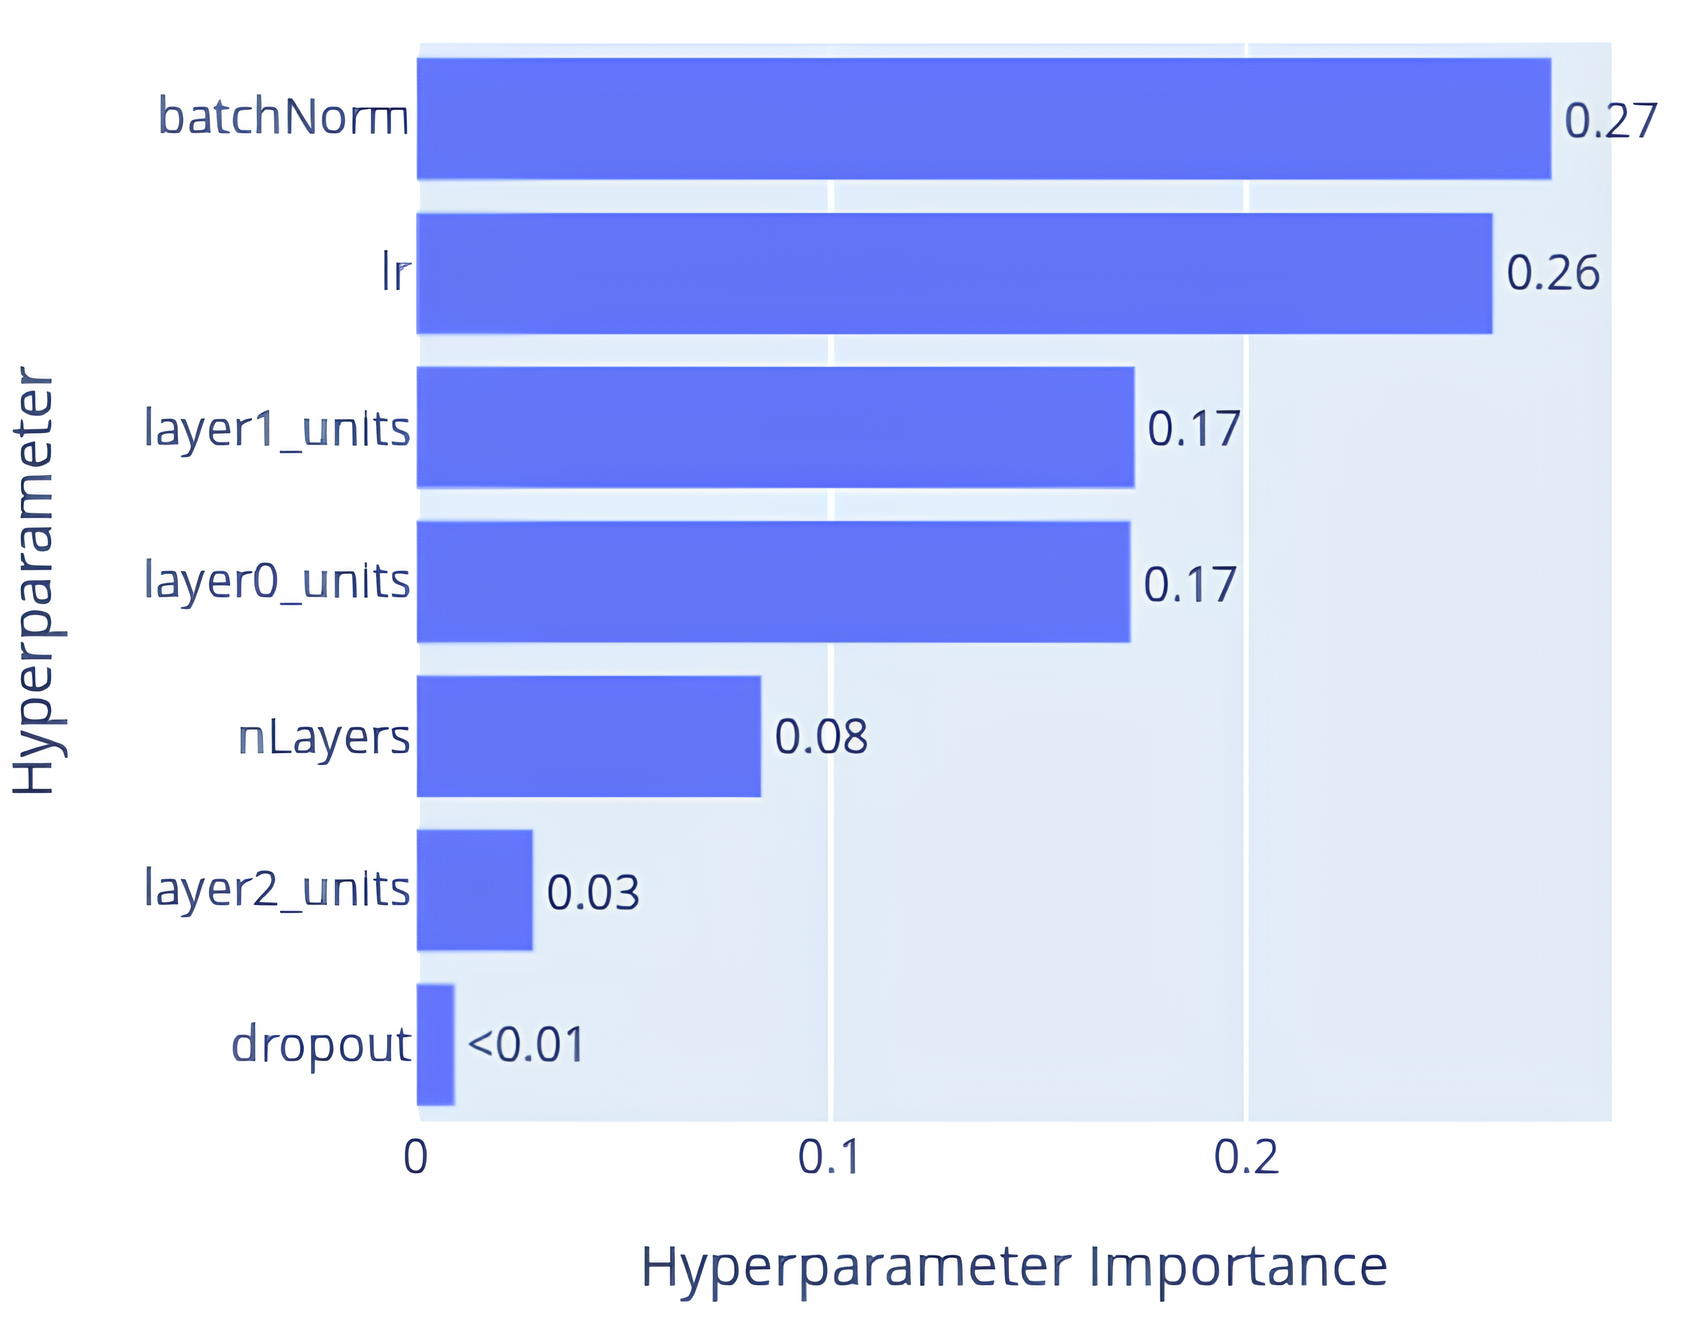
\includegraphics[height=.3\linewidth]{images/HP_importance.png}}\hfill
        \subfloat{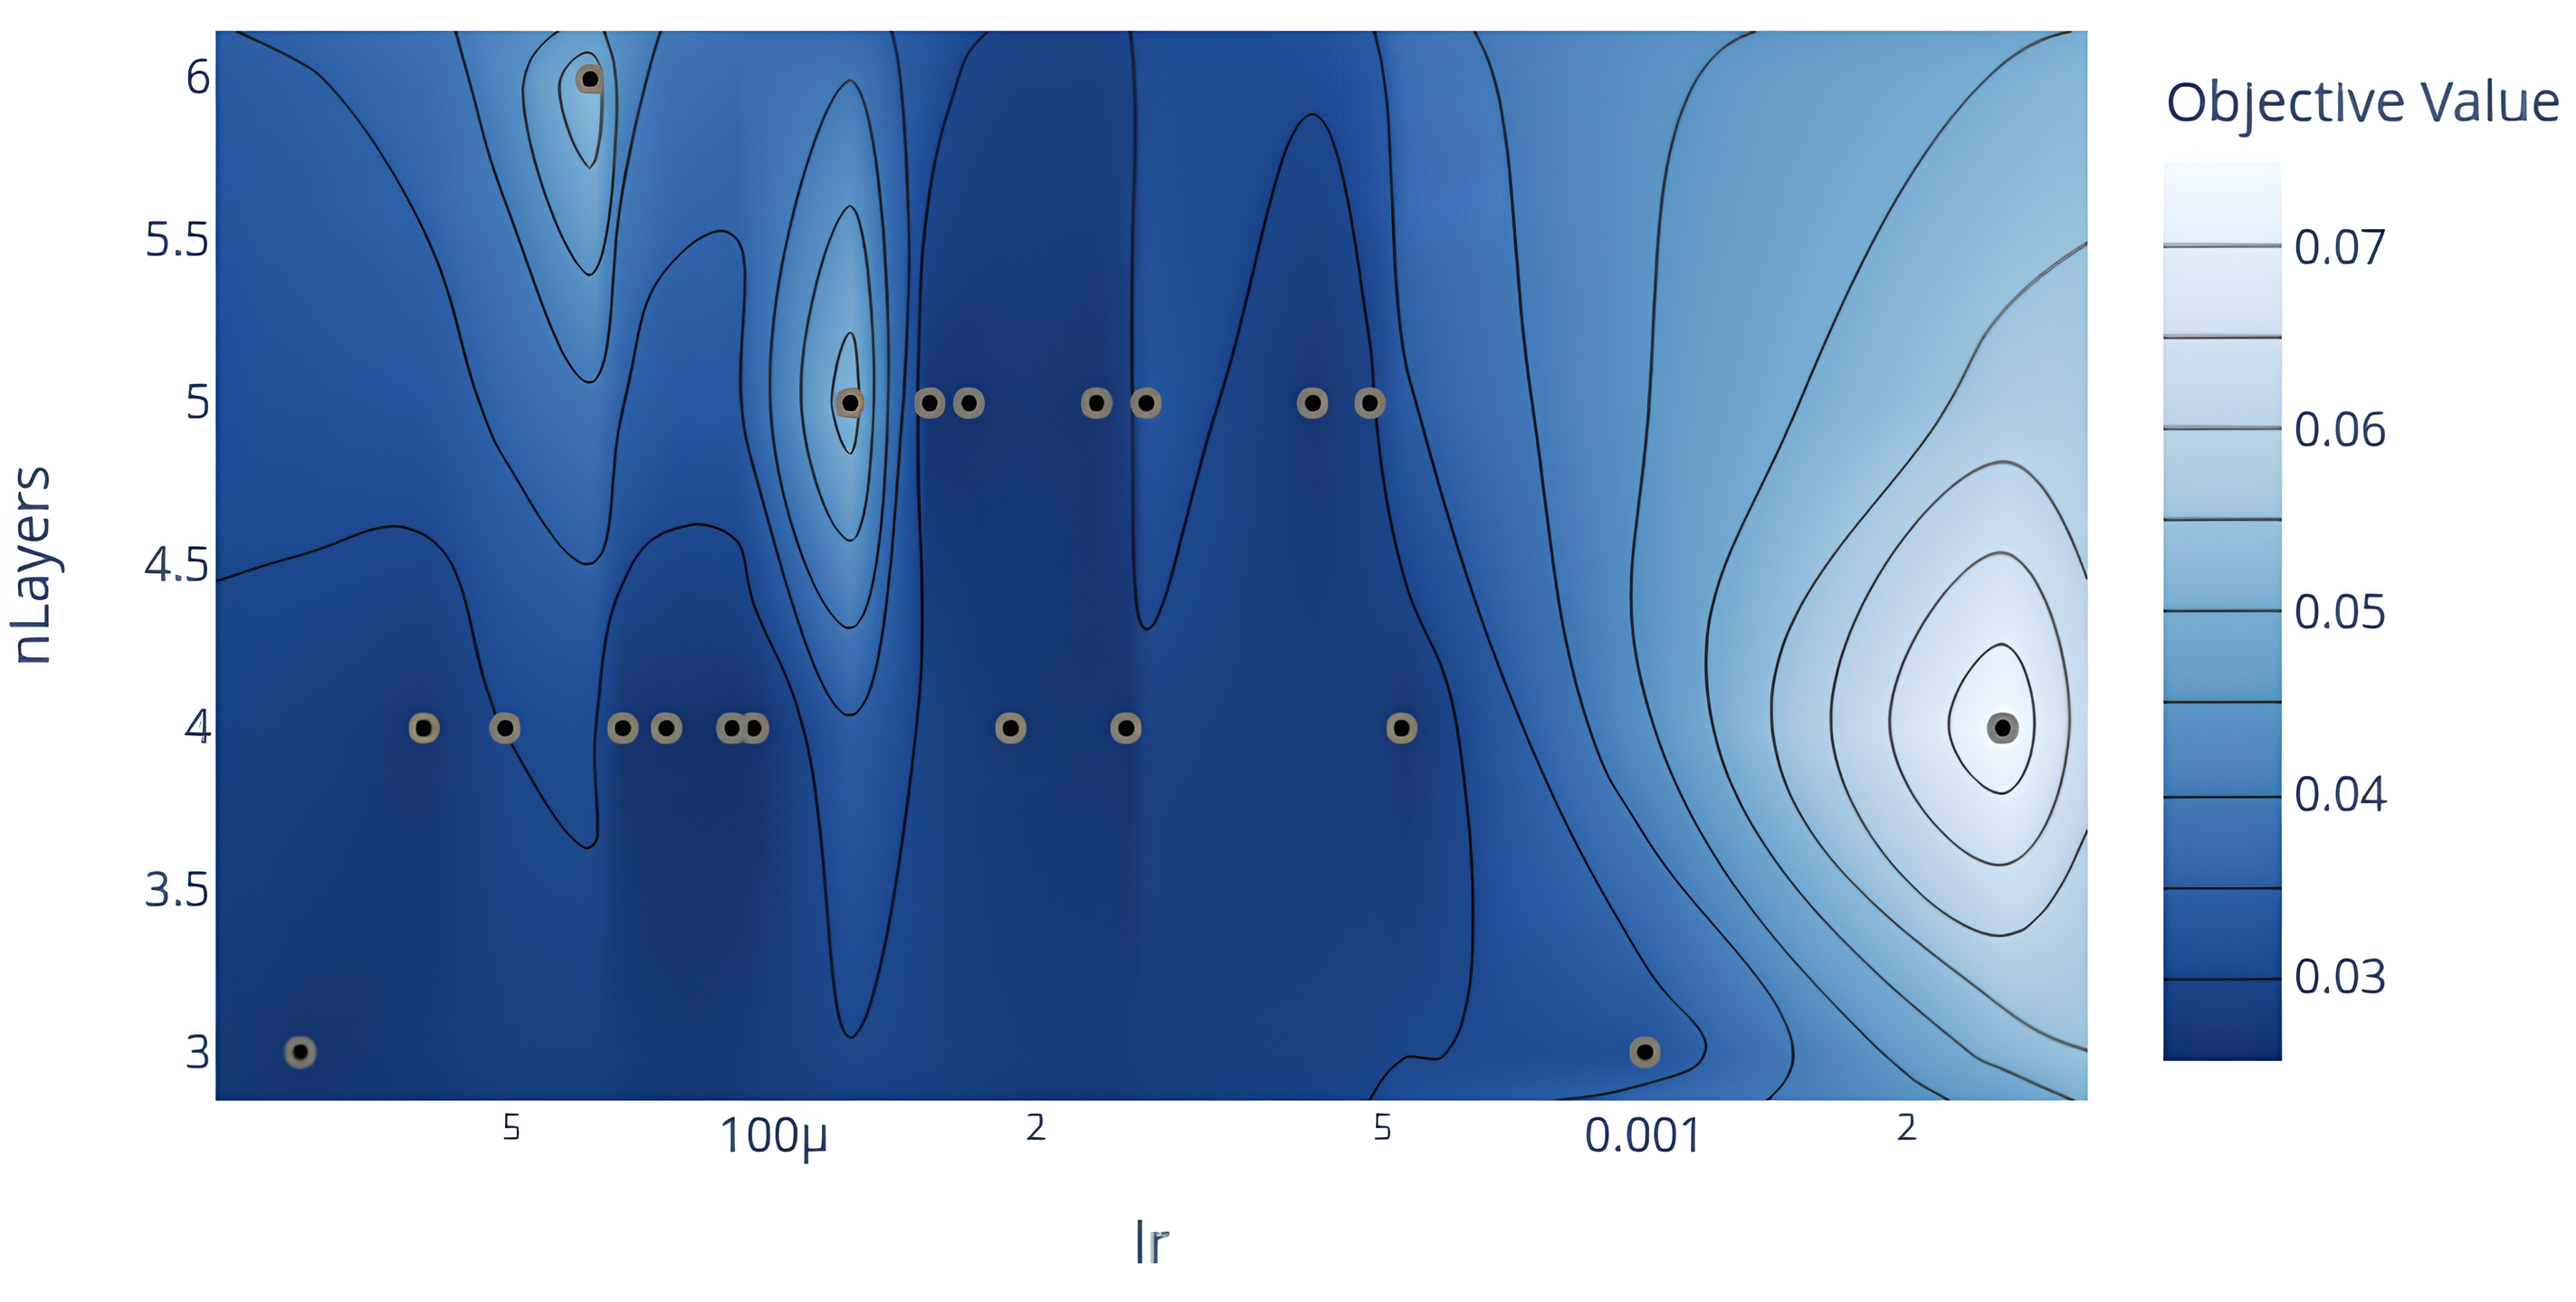
\includegraphics[height=.3\linewidth]{images/HP_contour_plot.png}}
    \caption{Relative importance and contour plot of the validation loss variation with respect to learning rate and  number of MLP layers.}\label{fig:HP_visualizations}
\end{figure}

\noindent
The list of tunable HPs, as well as their optimal values, is shown in \textbf{Table \ref{tab:HPselection}}, where we observe how the optimization process converged to some peculiar combinations of layers for the MLP head: for example, the EfficientNet head consists of five layers with [256, 256, 1024, 512, 512] units, which is a fairly unusual succession of layers. Moreover, for all architectures apart from ResNet, neither batch normalization nor dropout were used, which leads to models that converge very quickly to good validation losses, but tend to overfit for longer training runs, as described in the next section.

\begin{table}[ht!]
    \newcolumntype{Y}{>{\centering\arraybackslash}X}
    \begin{tabularx}{\textwidth}{YYYYY}
        \hline
                          & \textbf{Baseline}   & \textbf{ResNet}   & \textbf{EfficientNet} & \textbf{MobileNet} \\\hline 
          Learning Rate         & 1$e$-4        & 2e-4              & 5$e$-4                &  1.3$e$-3     \\ 
          Batch Norm.           & Yes           & No                & No                    &  No           \\ 
          Dropout               & No            & Yes               & No                    &  No           \\ 
          Dense layers          & 3             & 1                 & 5                     &  5            \\ 
          Units per layer       &[1024, 512, 128] & [1024]          & [256, 256, 1024, 512, 512]&[512, 64, 64, 64, 128]\\ \hline
    \end{tabularx}
    \caption{Manually selected HP (baseline) vs optimized HP.}
    \label{tab:HPselection}
\end{table}






%% OPTIMIZED MSE W/ CLIPPING
          %                 & \textbf{Baseline} & \textbf{ResNet} & \textbf{EfficientNet} & \textbf{MobileNet} \\\hline 
          % Learning Rate         & 1$e$-4 & 1.2$e$-5 & 1.4$e$-4  &  9.4$e$-5\\ 
          % Batch Norm.           & Yes   & No        & No    &  No\\ 
          % Dropout               & No    & No        & No    &  No\\ 
          % Dense layers          & 3     & 2         & 5     &  4\\ 
          % Units per layer       & [1024, 512, 128] & [512, 1024] & [512, 1024, 128, 64, 256]&  [128, 2048, 64, 512]\\ \hline




%%%% OPTIMIZED MAE W/out CLIPPING
          %                 & \textbf{Baseline}   & \textbf{ResNet}   & \textbf{EfficientNet} & \textbf{MobileNet} \\\hline 
          % Learning Rate         & 1$e$-4        & 8.5$e$-5          & 8.8$e$-4              &  1.3$e$-4\\ 
          % Batch Norm.           & Yes           & No                & No                    &  No\\ 
          % Dropout               & No            & No                & No                    &  Yes\\ 
          % Dense layers          & 3             & 5                 & 4                     &  4\\ 
          % Units per layer       &[1024, 512, 128] & [1024, 64, 64, 2048, 256] & [64, 64, 512, 128]&  [128, 512, 64, 128]\\ \hline